\documentclass[a4paper,12pt,twoside]{article}
\usepackage{IEM_2nd_Qtr}



\begin{document}

\thispagestyle{empty}

\begin{center}
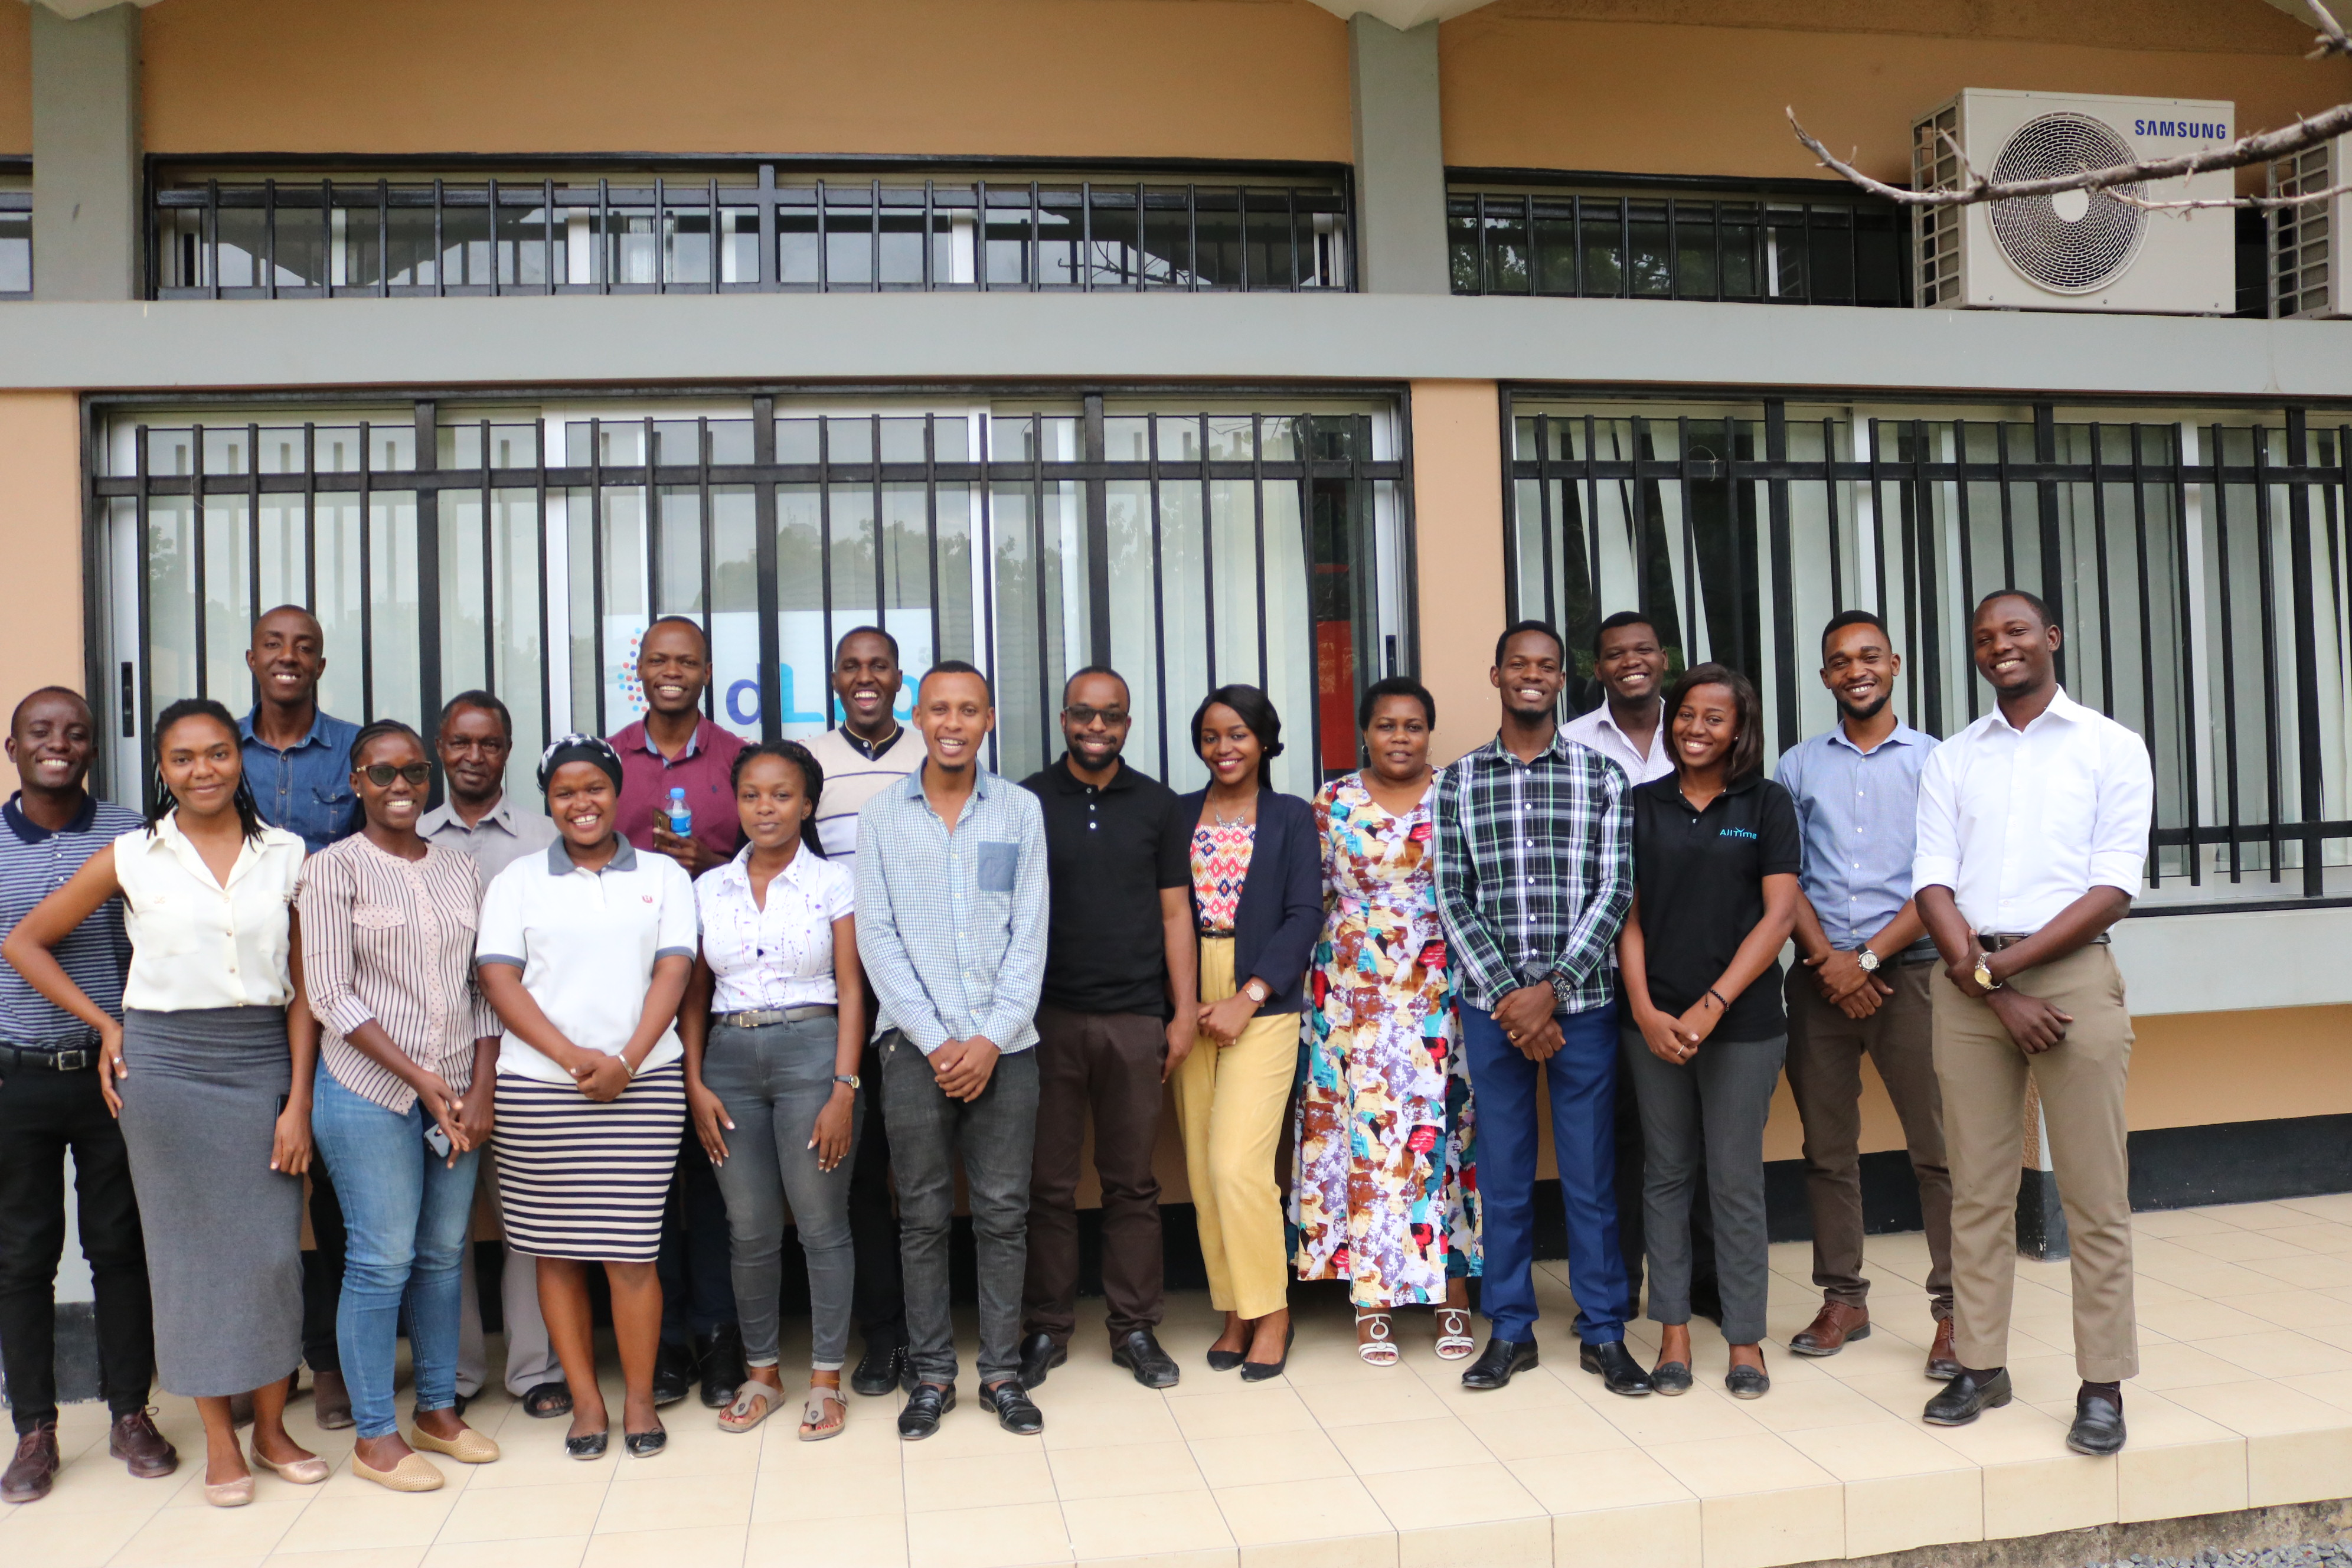
\includegraphics[width=\textwidth]{Group_shot.JPG}
\end{center}

\begin{center}
\bigskip
  \Huge 
\color{OMDTZblue} \textbf {Innovation Ecosystem Map}
\\
\textbf{Project Progress Report}
\\
\end{center}
\bigskip \bigskip \bigskip
\\
  \vbox{
  \centering
  Prepared for:
  \vcenteredhbox{
\includegraphics[width=2cm]{images/hdif_logo_new.png}}
  \
  by:
  \vcenteredhbox{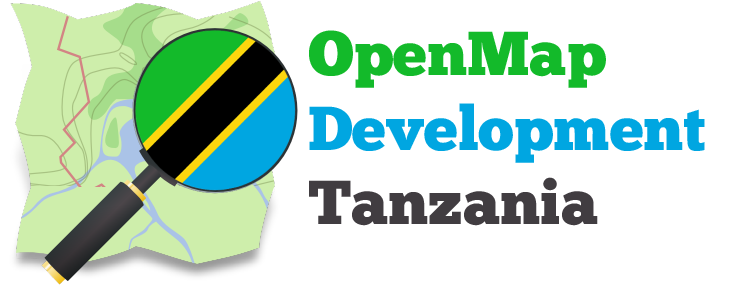
\includegraphics[width=4cm]{images/OpenMap_Development_TZ_Logo_Security_Card.png}}
  % \maketitle
}
\bigskip  \bigskip \bigskip
\begin{center}
  July 2019, Dar es Salaam, Tanzania  
  
 \bigskip \bigskip \bigskip \bigskip \bigskip \bigskip
\end{center}
 
\begin{flushleft}
	\footnotesize {\textbf{Authors:} Wombura Kimacha, Evarist Isdory, Johanes Peter, Hawa Adinani, Immaculate Mwanja and { } { } { } { } { } { } Innocent Maholi}
\end{flushleft} 
  

\newpage
\tableofcontents

\newpage
\section{Summary}
With the support from \textit{Human Development Innovation Fund (\href{http://www.hdif-tz.org/}{HDIF}\footnote{\url{http://www.hdif-tz.org/}}), OpenMap Development Tanzania(\href{http://omdtz.or.tz}{OMDTZ}\footnote{\url{http://omdtz.or.tz}})} has been tasked to review the technology and administer an innovation mapping platform as well as create community ownership of the platform by the innovation stakeholders in Tanzania. Administering the platform involves training innovation stakeholders to add relevant information to the map platform to facilitate collaborations and connect with each other to enable a conducive environment for innovators, for example, to interact with donors/funders or interact with fellow innovators to share experiences and work together in joint projects. Reviewing map technology involves making the map platform user-friendly and easy to interact with when using it.

Therefore, this report describes the second quarter of the Innovation Ecosystem Map of Tanzania Project and deep dives into the activities conducted in the quarter. It provides an in-depth description of the activities done from April to July of 2019 including web development for the newly developed map, training of the trainers responsible for training the innovation stakeholders in the country, mapathon held in Dar es Salaam, lessons learned so far from the engagement with stakeholders and the communication strategies for the sustainability of the Innovation Ecosystem Map of Tanzania.



\section{Milestones}
This section provides an overview of the project status with regards to activities conducted in the second quarter and their progress and milestones reached:

\subsection{Web Development}
Since the beginning of the second quarter, OMDTZ team has worked on developing a new mapping platform to replace the previous \textit{\href{http://innovate.co.tz}{innovation-map}\footnote{\url{http://innovate.co.tz}}} platform. Though a great mapping platform, the previous map had its own weaknesses. Through the internal team reviews and feedback from users during the innovation week 2019, the following were noted:

\begin{itemize}
    \item Inflexibility to filter innovation stakeholder features which makes it hard for beginner-users of the map to easily and efficiently use the map.
    \item As the map functions as the “market” for individual organizations/innovators seeking funds, the map had no ability to provide analytical functionalities to show traffic to the mapped features eg. who has visited your hub, when, etc.
    \item The display of results appeared in a long list format which sometimes made user go through several pages to find a particular result. This appeared to be an issue with users.
    \item Stakeholders want to know the state of the ecosystem through the platform. This would make it a one stop center for most of the information one will need from the innovation ecosystem of Tanzania. Information can be shared in various formats such as blog posts.
\end{itemize}

\begin{figure}[h]
    \centering
    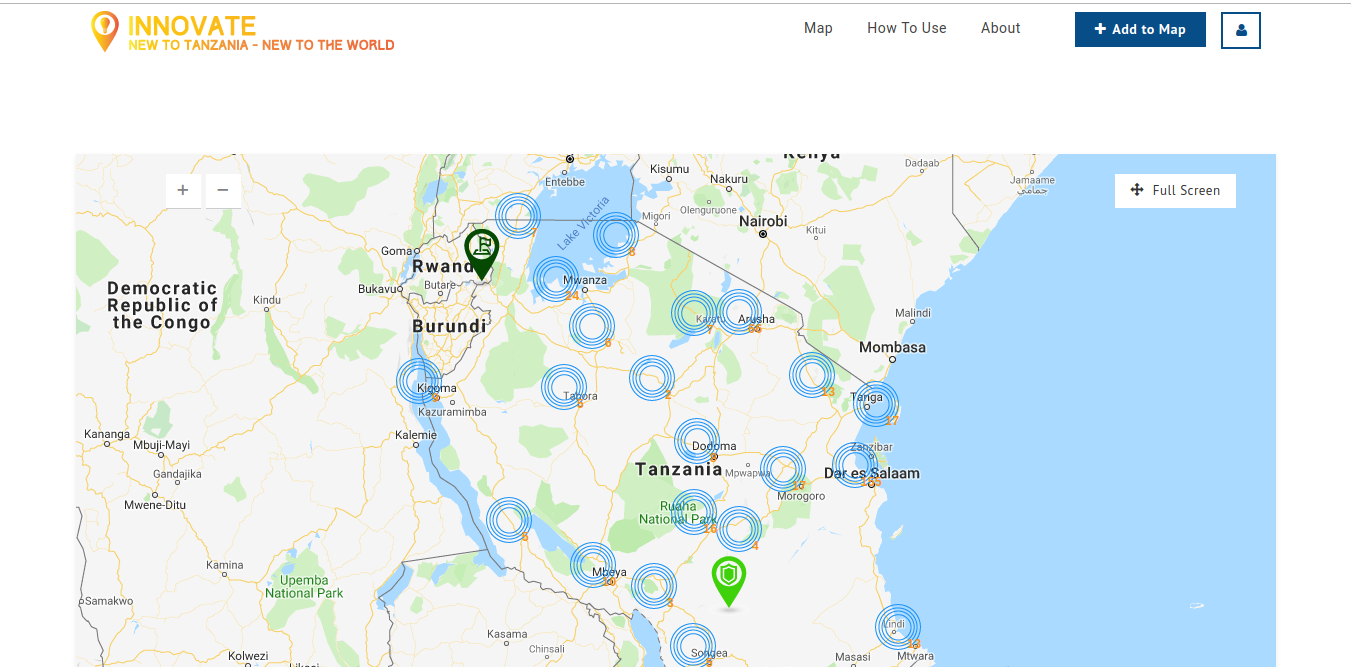
\includegraphics[width=0.9\textwidth]{old_inno_map.png}
    \caption{A layout of the old map platform on \href{innovate.co.tz}{innovate.co.tz}}
\end{figure}

With the aforementioned weaknesses, the development of the new mapping platform was carried out for a period of almost two months by the OMDTZ team. The following activities were done during this period:


\begin{itemize}
	\item Research for main layout
	
	This involved the process of decision making on what features are to be included in the platform and framing the structure of the website. User interface and experience inspired the final product.
	
	\item Concept generation, prototyping
	
	On the second week of May, 2019 concept generation enabled us expand our range of ideas for the new platform development. Several ideas where generated while considering user  experience. First prototype was released on the third week of May, 2019 and a second on the fourth week of May.
	
	\item Development, and lots of internal reviews to gain feedback and improve the platform
	
	On the first week of June, 2019 development of the new map started along with frequent internal meetings. These provided feedback which was constructive to the development of the platform. Things which were discussed during the meetings included branding strategies and blog posts.
	
	\item External review with the HDIF which also helped improve the platform
	
	During catch-up meetings with HDIF, we were able to receive various feedbacks for the platform such as which branding content should be used for the map. On the 21st of June, 2019 the new map was submitted during the meeting for reviews. Among the feedback we received was to not use the abbreviation IEM (Innovation Ecosystem Map) on the website due to confusion with other brands on the internet like Institution of Engineers, Malaysia.
\end{itemize}

The development of the new platform passed several reviews internally and externally. This was meant to improve the user experience and simplify how innovators will be able to use the platform. In the fourth week of June, the new platform was completed awaiting reviews from the innovation stakeholders that attended the Dar es Salaam mapathon. The new map is now live and \href{http://new.innovate.co.tz}{accessible}\footnote{\url{http://new.innovate.co.tz}}

\begin{figure}[h]
	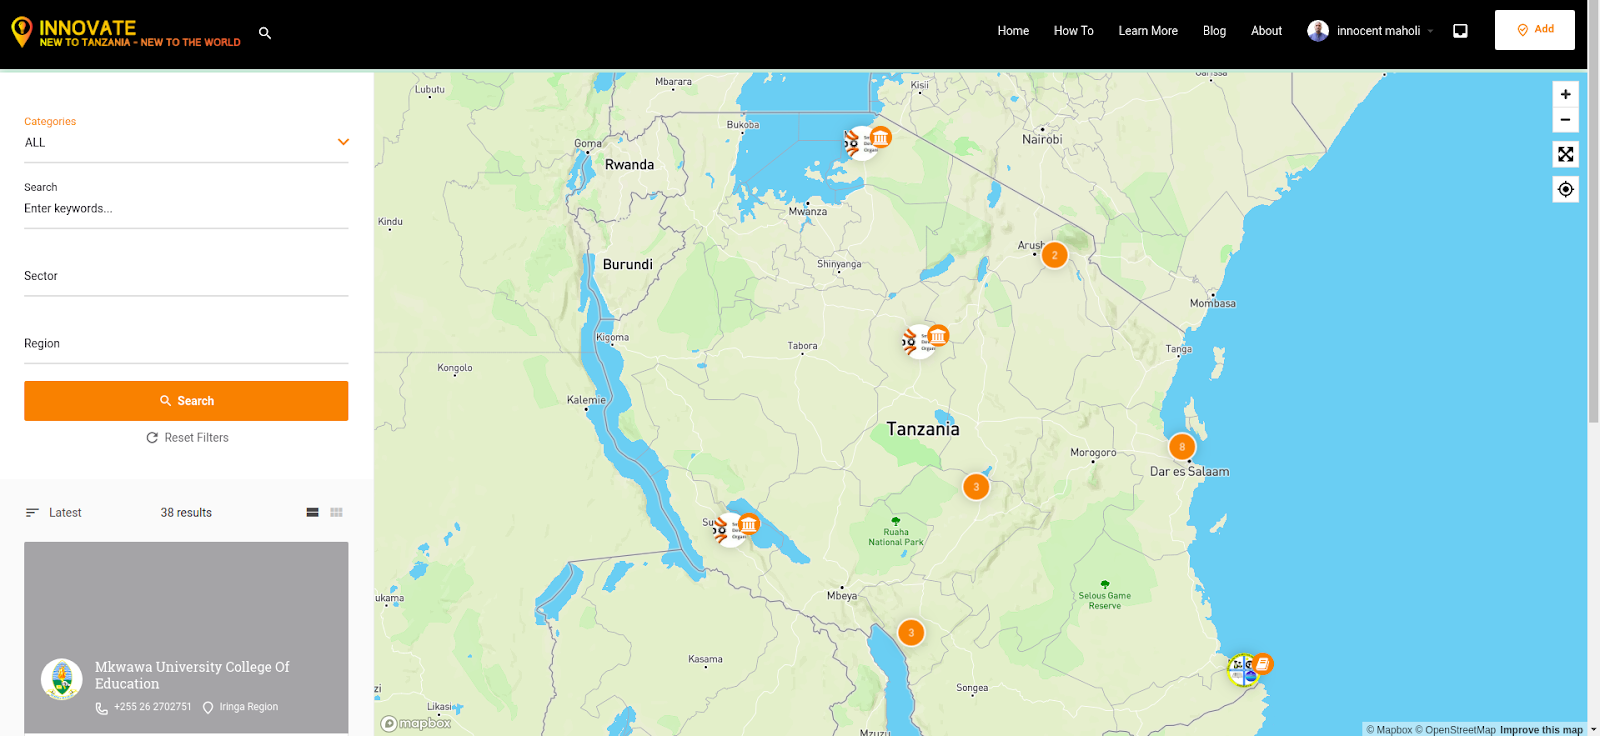
\includegraphics[width=0.9\textwidth]{images/new_new_inno_map.png}
	\caption{A layout of the new map platform on \href{http://new.innovate.co.tz}{new.innovate.co.tz }}
\end{figure}
\begin{figure}[h]
	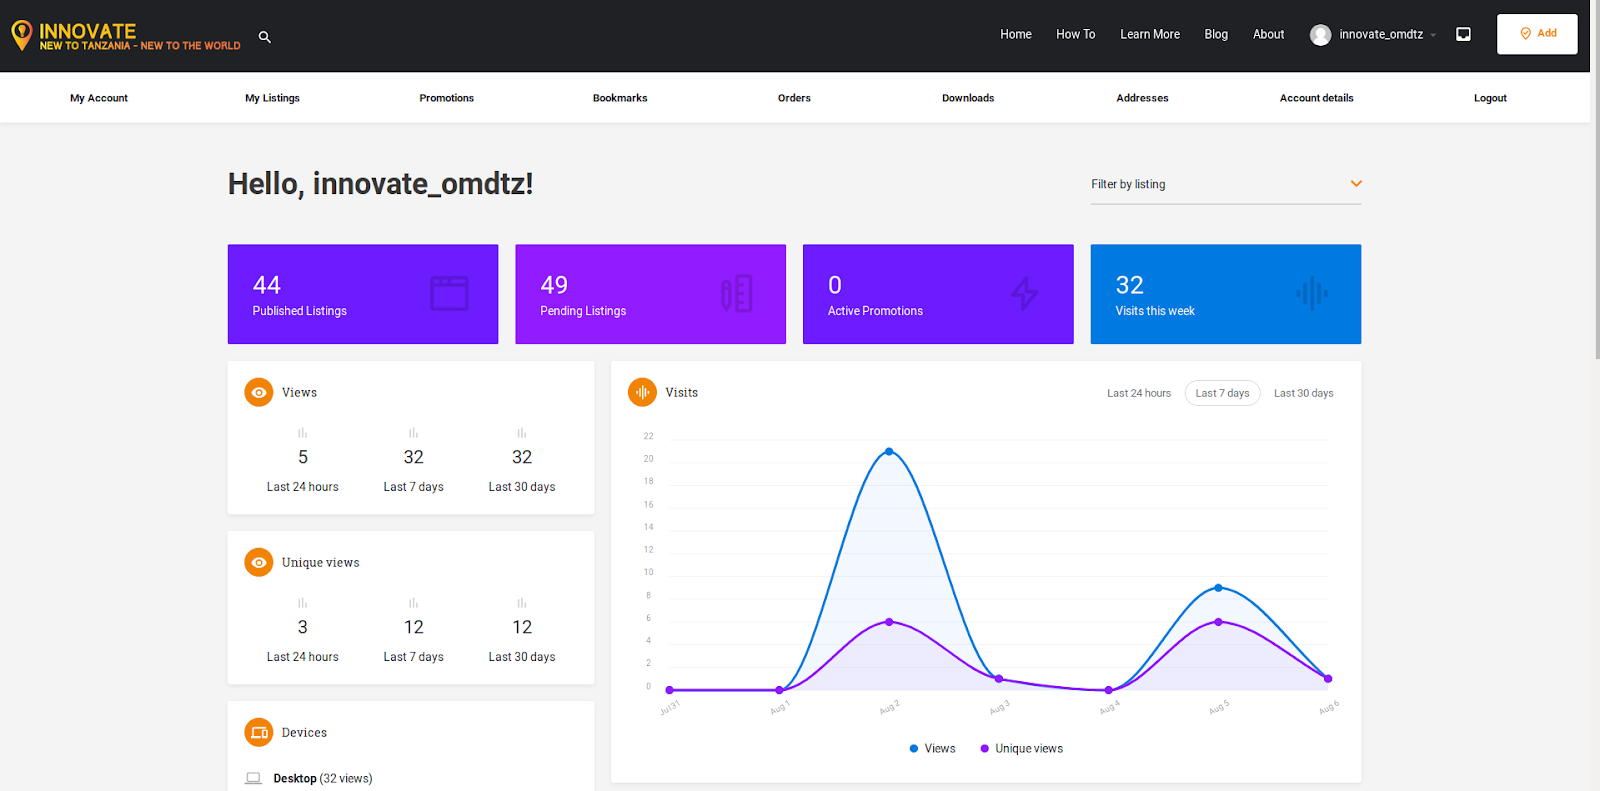
\includegraphics[width=0.9\textwidth]{images/dashboard.png}
	\caption{A layout of the new map platform user dashboard showing feature analytics }
\end{figure}

The new mapping platform was developed by using a \textbf{WordPress content management system.} It has an advanced filtering option compared to the previous map which makes it easier for the user to get desired results. It offers a page for instructions on how to use the map so that any new user won't have issues trying to navigate the map. A blog is another new section offered where different posts about the activities and state of the innovation ecosystem will be shared.

\subsubsection{Challenges and Lessons Learned}
The development of the platform took a much longer time to complete as a result of feedback from meetings between internal staff and our clients. Changes to the development of the platform were inevitable and we took the suggestions optimistically. Internal meetings provided reviews on the new platform focusing on user experience and interface. Therefore, they provided improvements for the new platform.

Once the website was completed, we reached out to the HDIF team to present and review the new platform. Reviews from the meeting that we had on the 21st of July, 2019 indicated that the new platform was accepted for the task. After a few days, we received requests from Simon to include more features which the current platform could not handle. Due to that---even though the days to the mapathon were numbered---there was an instruction to create another platform to address the issues presented which led to shifting the focus on development of a new platform with added features such as further analysis of the entries, matchmaking for the stakeholders and storage of migration data points to be visualized.

On the 4th of July, 2019 we had a call with Nate from the Humanitarian OpenStreetMap Team to discuss about the capability of the current platform to include features such as overlaying more layers of data for analysis, storing information changesets and matchmaking features. Through the discussion, it appeared that the new platform could not incorporate these features. Further discussions were held with various developers including Hype Interactive and Tehama lab. 

On 31st July 2019, we had a meeting with the HDIF team to discuss the development of the new platform as explained in the terms of reference for its development.


All suggestions provided in the reviews were for a good cause and improvement of the user experience and interface. As a result of frequent changes to the design of the platform, we did not get enough time to populate the map with stakeholders’ information as agreed. The map is going to be populated with data from both old platform and the new one. The task will be done by our mappers with 2 weeks of importation of data from the old platform and continuing with the collection of new data. Currently, the platform seems to be loading slowly and we believe that it is due to it being a subdomain of the old platform (hosted on the same server).

\subsection{Training of Trainers}
The OMDTZ team in collaboration with the HDIF team conducted a training-of-trainers that took place on July 15th, 2019 at OMDTZ offices in Mikocheni. The main objectives were to train mappers on how to conduct innovation mapathons and introduce them to travel guidelines that should be followed while in the fields in the country as well as to give them training on supervision of work to conduct mapping of the Innovation Ecosystem Map of Tanzania.

Following the training that was provided in January 2019, the trainers were already familiar with the categories and contents of the Innovation Ecosystem of Tanzania. The training was collaborative as it provided room for interaction for every participant to air out their questions and comments on the stakeholders, categories, sub-categories, and targeted groups on the map.  

It mainly focused on training the trainers who will be going out to the field all over Tanzania to hold mapathons and/or workshops with hub managers, innovators, teaching institutions, etc. in order to populate the developed map.

\begin{figure}[H] % uncomment "[H]" to force the  image to the middle of the page  
	\centering
	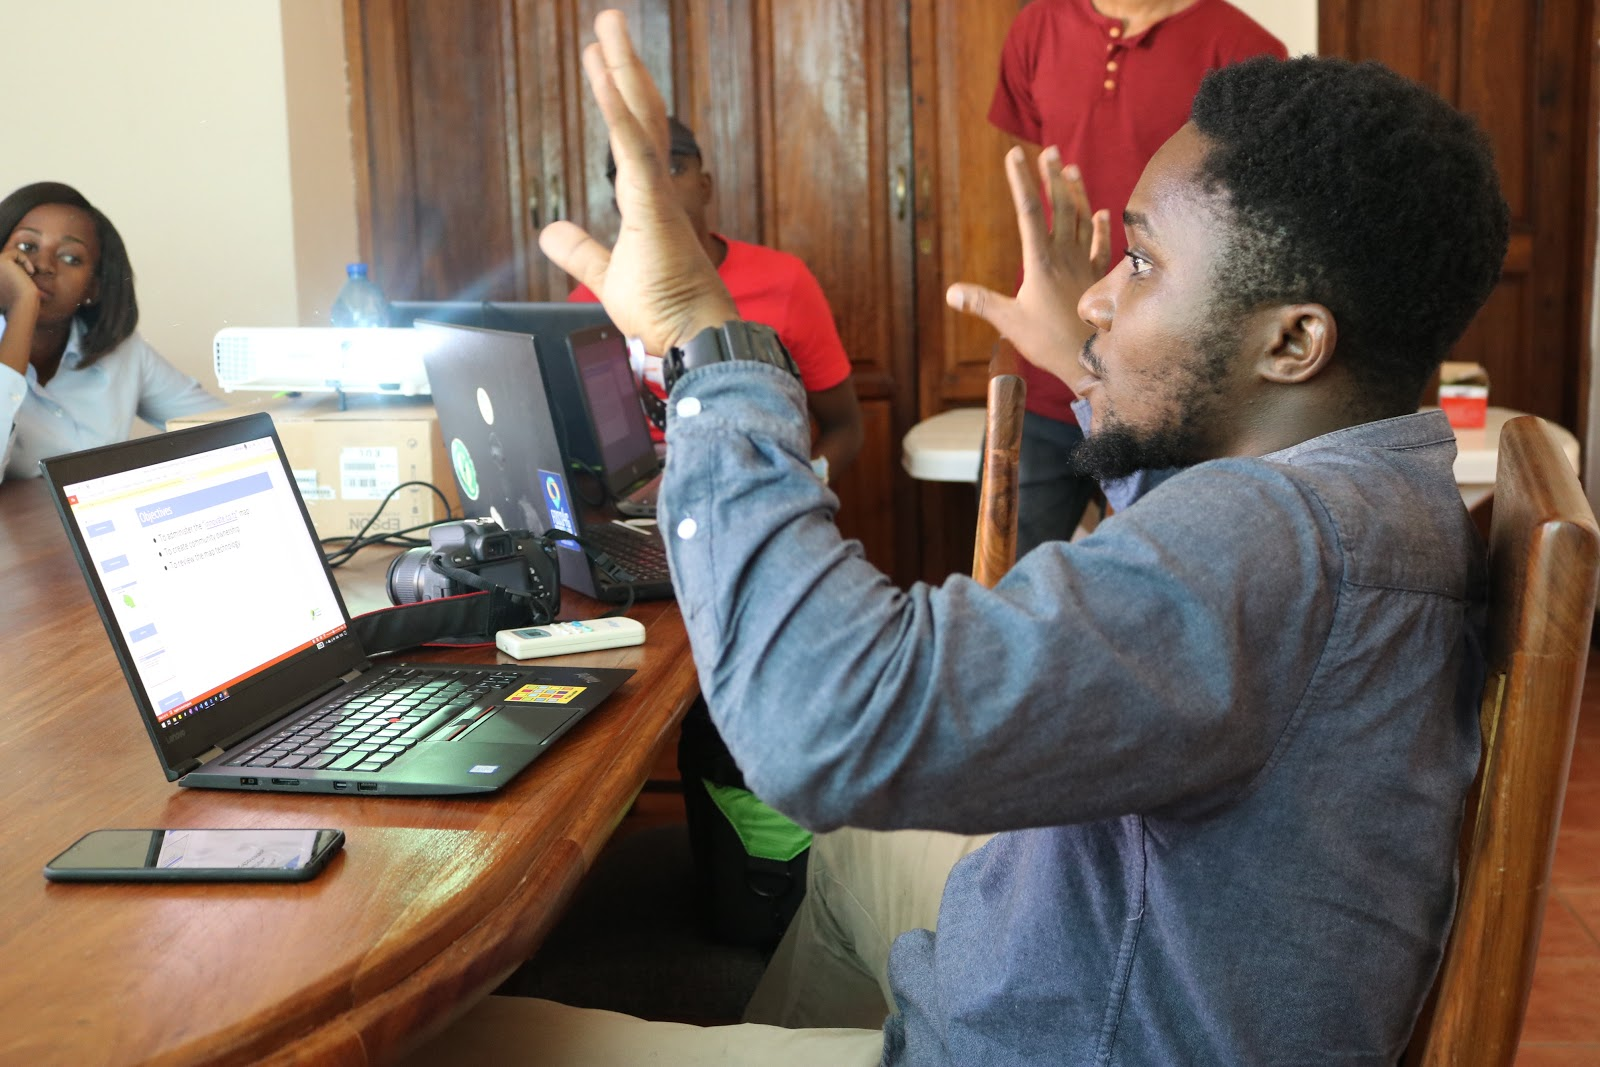
\includegraphics[width=0.8\textwidth]{images/Simon_training.JPG}
	\caption{Simon Mtabazi from the HDIF team commenting on the training of trainers held at OMDTZ office}
\end{figure}

The focus of the training was based on:

\begin{enumerate}
	\item Introducing the trainers to travel guidelines that will be followed when in the fields across the country.
	\item How to plan and conduct mapathons with the involvement of innovation stakeholders in districts and regions of Tanzania
	\begin{enumerate}
		\item How to register stakeholders and adding the listings of their categories
		\item Facilitate stakeholders in conducting their own mapathons and workshops that will be attended by the innovation stakeholders that could not be reached by the trainers
	\end{enumerate}
	\item Introducing the trainers to the web map developed for the innovation ecosystem of Tanzania
\end{enumerate}

The training of trainers was succeeded by a mapathon that was conducted the next day on July 16, 2019.

\subsection{Mapathon}
Before the mapathon, an \href{https://innovationtz.eventbrite.com}{Eventbrite page}\footnote{\url{https://innovationtz.eventbrite.com}} was created for participants to register and get their tickets as a notice in order for the OMDTZ team to coordinate and prepare the event. This was then shared through OMDTZ’s and Innovation TZ’s social media channels as well as shared with the labs and hubs, universities and physical innovation spaces in Dar es Salaam that would participate in the mapathon. A total of 25 participants registered to attend the mapathon.

On 16th July, the OMDTZ team with support from the HDIF and the \textit{\href{https://dlab.or.tz/}{Tanzania Data Lab (dLab)}\footnote{\url{https://dlab.or.tz/}}} teams hosted the first innovation mapathon that took place at the dLab training room. 

\begin{figure}[H]
	\centering
	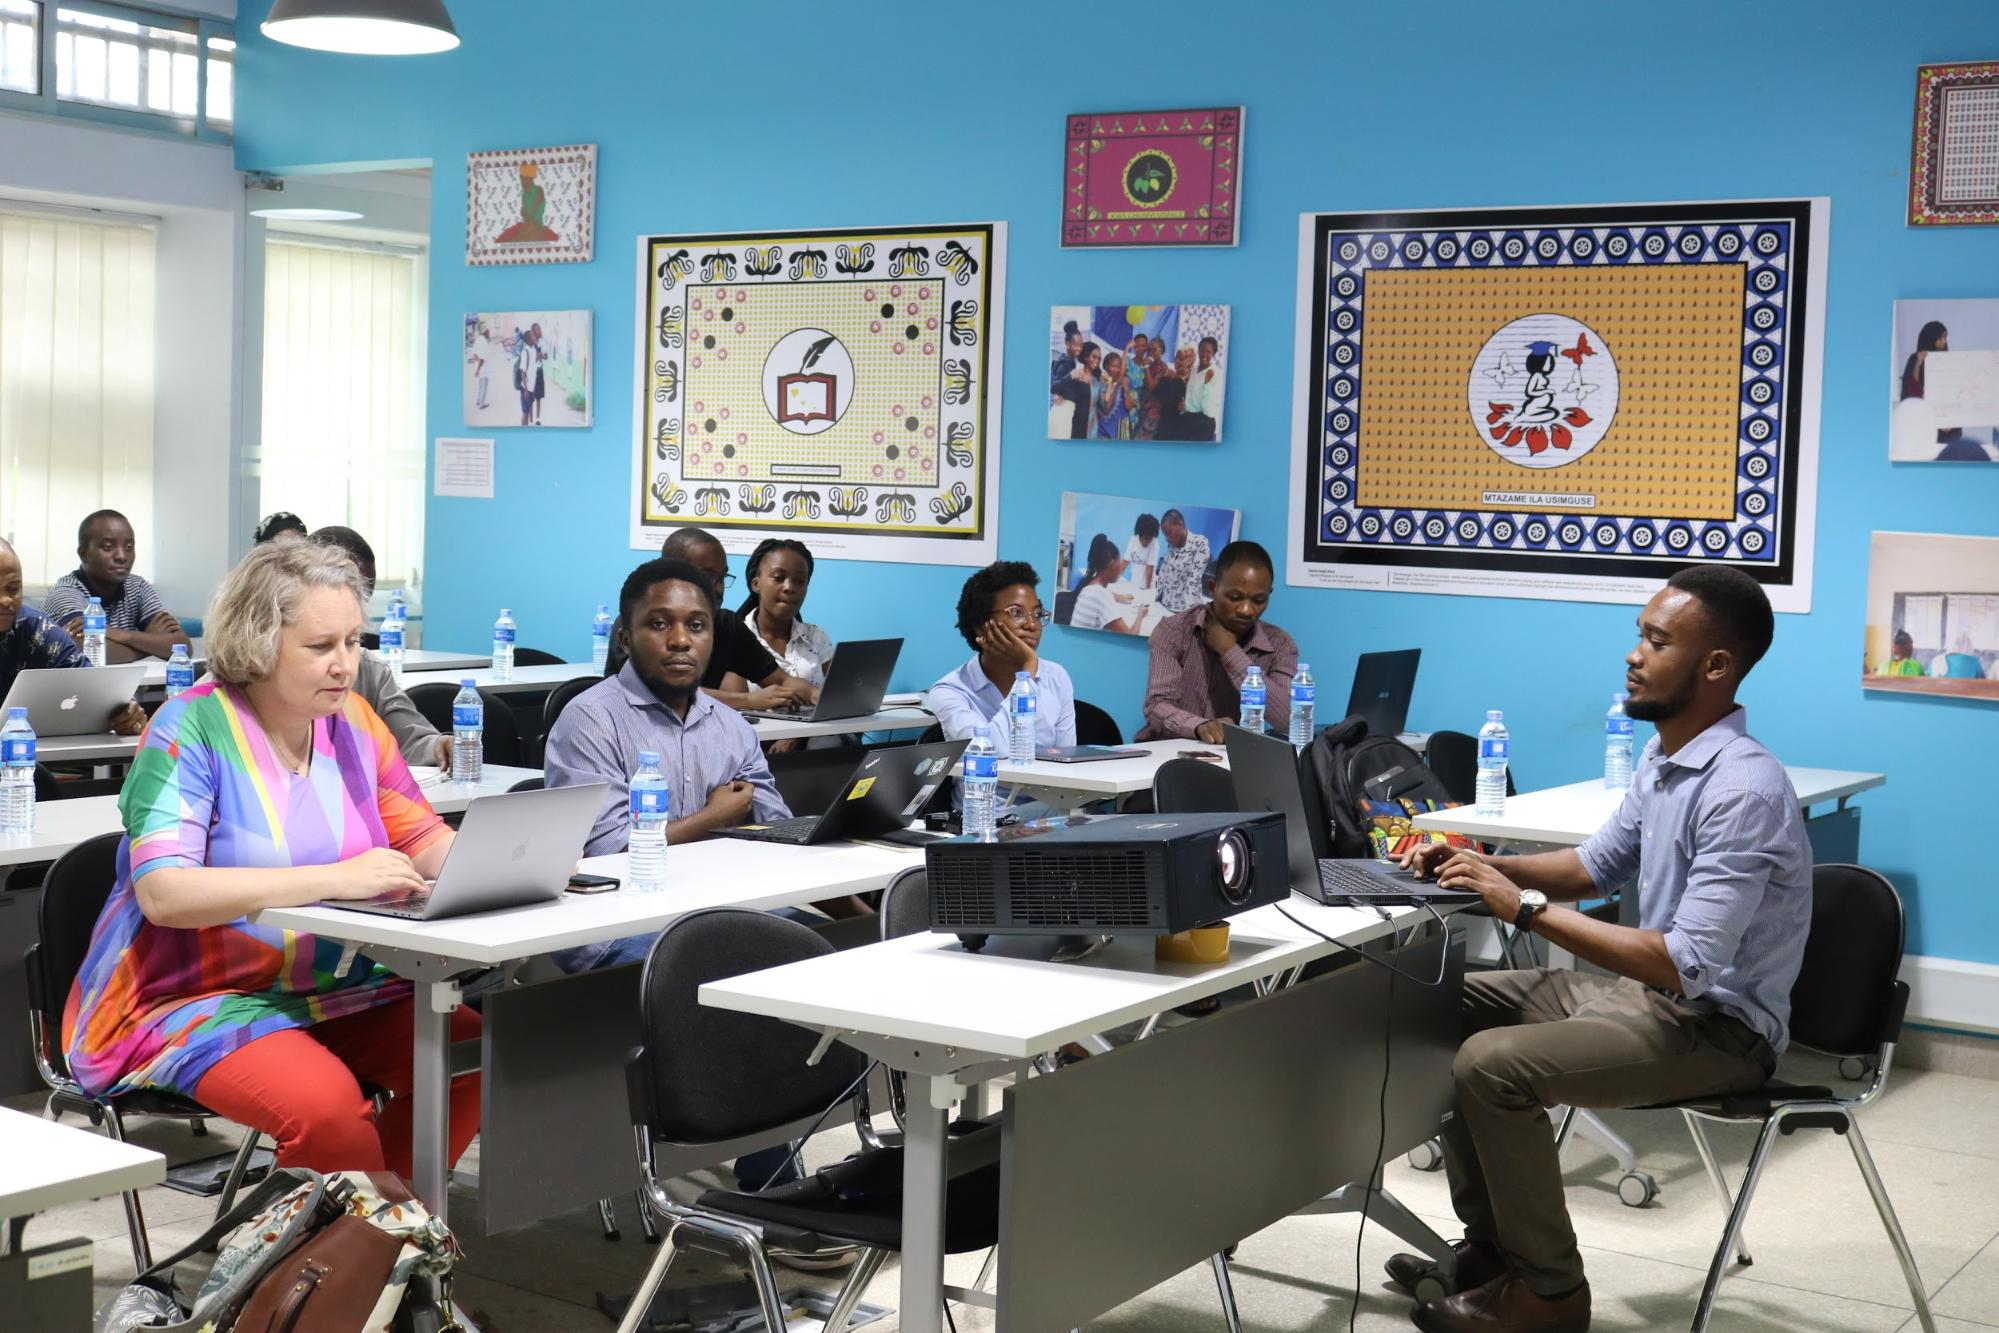
\includegraphics[width=0.8\textwidth]{mapathon.jpg}
	\caption{Mapathon conducted at Tanzania Data Lab}
\end{figure}

\subsubsection{Attendance}
Even though 25 people registered for the mapathon, according to registration only 14 people attended from various innovation organizations based in Dar es Salaam and Arusha. The participants were of different gender, as below;

\begin{figure}[h]
	\centering
	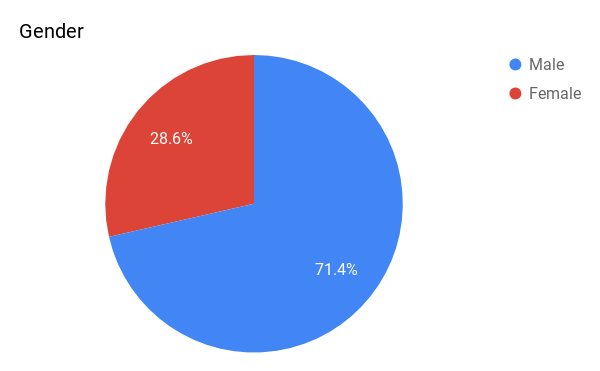
\includegraphics[width=0.6\textwidth]{Gender_chart.png}
\end{figure}

\subsubsection{Content}
The mapathon took approximately a maximum of 3 hours and was largely designed to introduce the participants into the innovation platform where the participants received full training on how to map themselves and used the time to actually map their organizations. The timetable for the mapathon is as below;

\begin{tabular}{|c|c|c|c|}
	\hline
	\rowcolor{Gray}
	\bfseries Time & Agenda & Responsible Person(s)\\
	\hline
	10:00 am - 10:20 am & Registration & All\\
	\hline
	10:20 am - 10:25 am & Welcoming Note & Innocent - OMDTZ team\\
	\hline
	10:25 am - 10:40 am & Introduction to and background of & Simon - HDIF team\\
	{} &  the Innovation Ecosystem Map & {}\\
	\hline
	10:40 am - 11:00 am	& Presentation of the map categories & OMDTZ trainer(s)\\
	\hline
	11:00 am - 11:20 am & Mapping Training & OMDTZ trainer(s)\\
	\hline
	11:20 am - 12:00 pm & Mapping exercise & All\\
	\hline
	12:00 pm - 12:20 pm & Feedback session & All\\
	\hline
	12:20 pm - 12:30 pm & Closing & All\\
	\hline
	12:30 pm - 1:00 pm & Lunch and Networking & All\\
	\hline
\end{tabular}

During the mapathon, the OMDTZ team provided an in-person consultation to the participants to help them with using the map platform and be able to add themselves on the map.
\begin{figure}
	\centering
	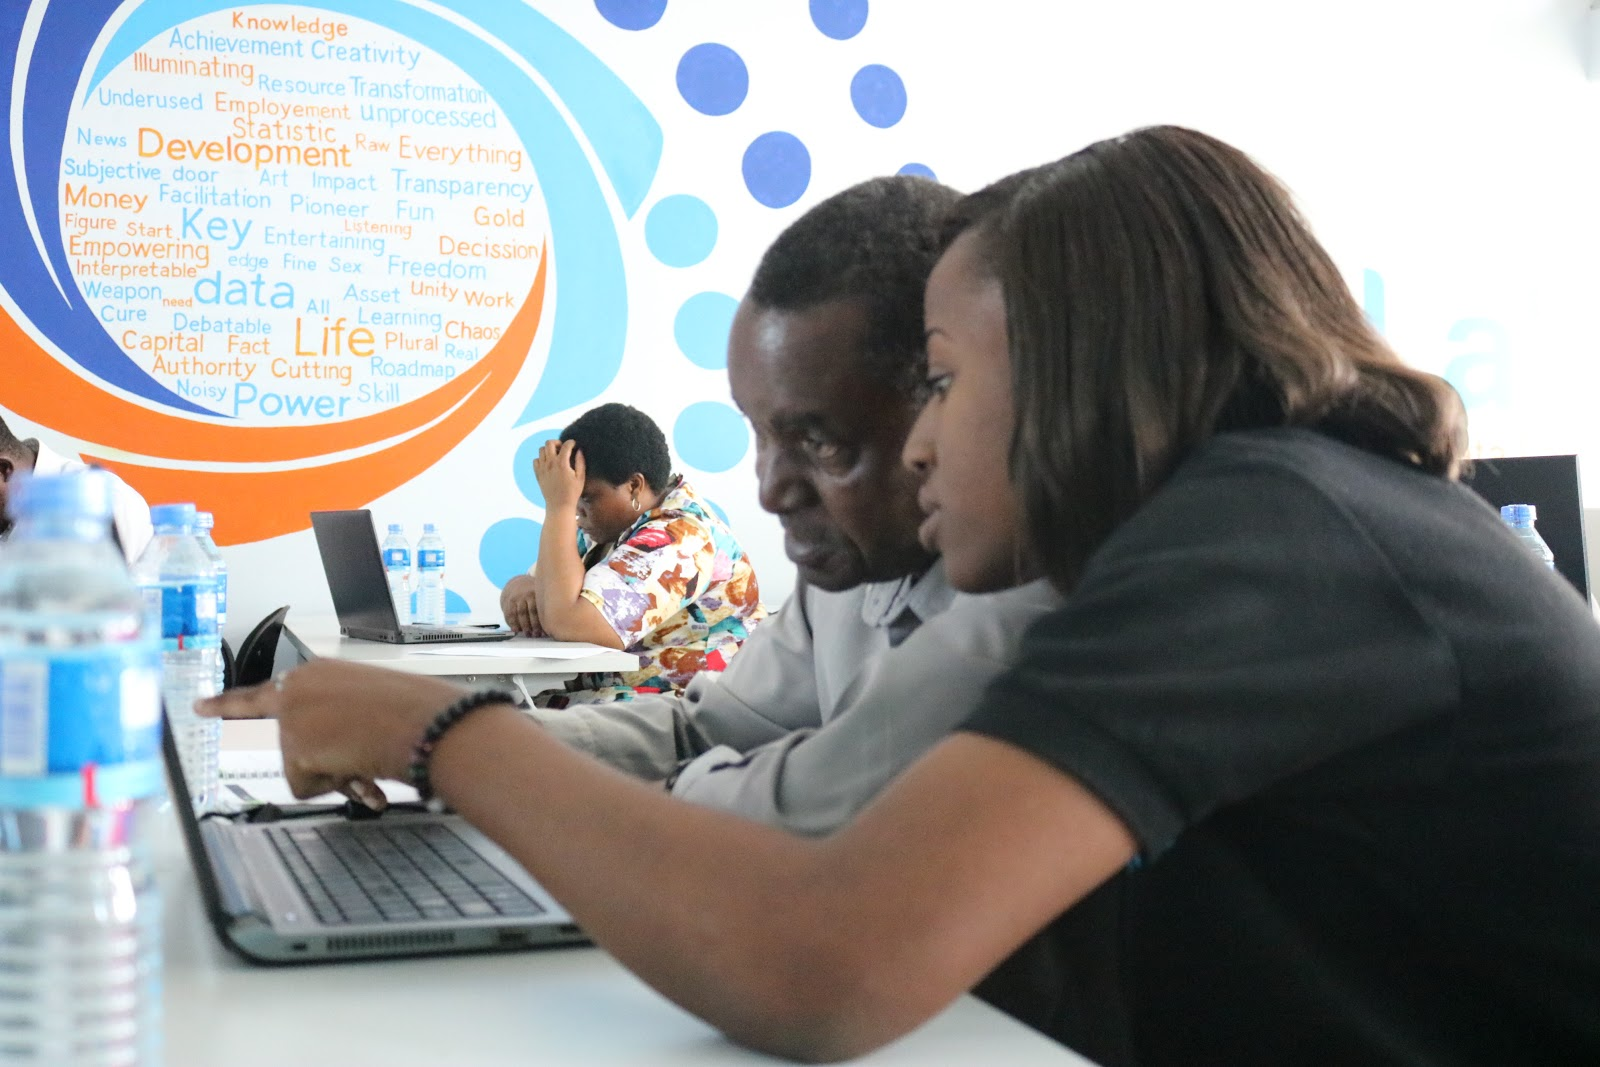
\includegraphics[width=0.6\textwidth]{mapathon_instruction.JPG}
	\caption{OMDTZ trainer helping the participant to add their organization on the map}
\end{figure}

\subsubsection{Feedback}
What the OMDTZ team learnt from the mapathon is that most of the participants were familiar with the new map being developed by OMDTZ from the Hubs Manager’s workshop, exhibition, and presentations held during the Innovation Week of 25th - 30th of March, 2019. Regardless, the participants were able to provide their feedback on the mapathon and the map platform;

\begin{tabular}{c|c|c}
	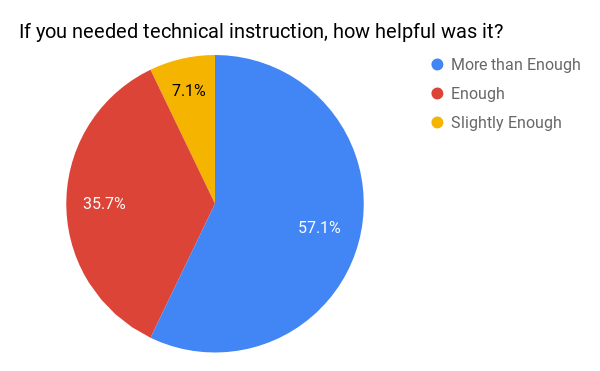
\includegraphics[width=0.5\textwidth]{Instructions_chart.png} 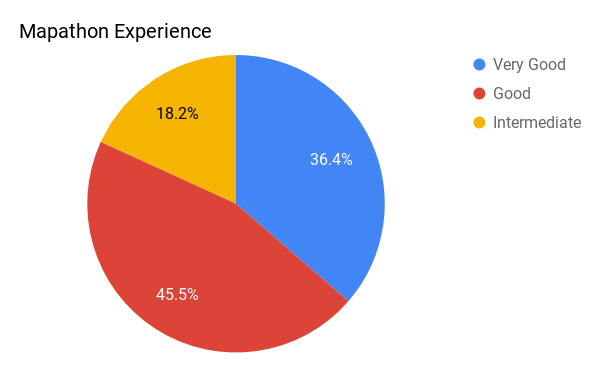
\includegraphics[width=0.5\textwidth]{experience_chart.png}\\
	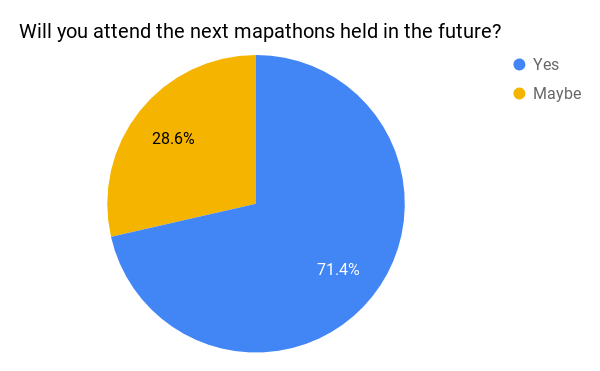
\includegraphics[width=0.5\textwidth]{future_attend_chart.png}\\
\end{tabular}

The participants were able to give a few recommendations to improve the future mapathons and the map platform, some of the recommendations are as follows;

\begin{enumerate}
	\item Work around on the more features that will help get more locations and please remove the Brela certificate and allow the people to reviews the available locations that one will provide more data and help more use case. Thanks to Angela (OMDTZ trainer) she was so helpful in explaining.
	\item You need to have stable internet Wi-Fi so we can move faster. I do congratulate you guys for challenging existing map. Well done
	\item I suggest that the team reaches out to more targets who could be part of the ecosystem like university students, participating companies and others.
	\item To invite more stakeholders
	\item The user experience should be improved, filling in information shouldn't be a very long process, you should try to catch a few pieces of information which are vital, for example other information a particular company can be found on their website
\end{enumerate}

\subsubsection{Challenges and Lessons Learned}
For the second quarter, our work plan showed that 3 mapathons were to be conducted in Dar es Salaam, Arusha and Dodoma. One mapathon was conducted in Dar es salaam successfully on July 16th but we were not able to do the other two mapathons. This was a result of the feedback we received from the attendants of the event. We decided to cancel other mapathons and focus on fixing issues that we experienced with the new map platform such as crashing of the web platform. Currently, most of the comments that we received during the mapathon have worked.

Other challenges that were experienced during the mapathon include:
\begin{itemize}
	\item {\color{OMDTZblue}Internet connection:} During the beginning of the mapathon, the internet connection was poor but became stable as time went on. This caused a delay in some of the activities. In the next mapathons that will be conducted, we shall strive for a more stable connection and test it before we commence.
	
	\item {\color{OMDTZblue}Venue of the mapathon:} We delayed in booking the venue for the mapathon which posed as a challenge as we could not find a reliable (cost effective) venue at the very last minute with the limited time that we had left. In the future mapathons, a proper research on which venue should be used during mapathons will be conducted earlier and the booking will be done on time in order to avoid any future inconveniences.
	
	\item {\color{OMDTZblue}Attendance to the mapathon was lower than expected:} This is because invites to the attendees were sent later than our goal . Invites need to be sent at least 1 month before the event---with frequent reminder to the invitees---so they are aware of the upcoming events and can schedule their timetables accordingly.
\end{itemize}

\section{Communications}
Communicating to the public about the innovation map is the focus and the OMDTZ team is committing to make that happen. The OMDTZ team has prepared a \textit{\href{https://docs.google.com/document/d/1E2_zR-vNxvte00CZwfj4i6A3WDjTw4HnVKfInVP6lpE/edit?usp=sharing}{draft communication strategy}\footnote{\url{https://docs.google.com/document/d/1E2_zR-vNxvte00CZwfj4i6A3WDjTw4HnVKfInVP6lpE/edit?usp=sharing}}}---just for the map---that both teams from HDIF and OMDTZ are reviewing to finalize. The strategy will guide all communications about the project and the type of content to be shared with the public.

The \textit{\href{https://docs.google.com/document/d/1fQhdXPWNA6JcoFd8slqdueiZXXzb1eEI5t2ZXrlZ72g/edit?usp=sharing}{blog draft}\footnote{\url{https://docs.google.com/document/d/1fQhdXPWNA6JcoFd8slqdueiZXXzb1eEI5t2ZXrlZ72g/edit?usp=sharing}}} has been developed but not published yet as we are still waiting for reviews from the HDIF's communications specialist. This will be published as soon as the communication strategy is finalized.

Also, during the innovation week, we had an opportunity to publicise the map to stakeholders through mainstream media coverage on two platforms---\href{https://youtu.be/o5rtxjeeLVI?t=55}{BBC News Swahili in Mitikasi Leo Show}\footnote{\url{https://youtu.be/o5rtxjeeLVI?t=55}} and ITV news (unfortunately, they could not upload the coverage to YouTube but the session was aired on the evening news)---where we introduced the map and explained why HDIF is interested on this platform and how it will be useful to the innovation ecosystem of Tanzania.

\subsection{Social Media}
Handling multiple social media accounts is challenging especially when the accounts are not popular yet, therefore, in order to create good and reliable contents, we decided to create only two social media accounts as a starting point. These were;

\begin{enumerate}
	\item Facebook page - \href{https://web.facebook.com/innovatetz}{innovatetz}\footnote{\url{https://web.facebook.com/innovatetz}}
	\item Twitter account - \href{https://twitter.com/innovate_tz}{innovate\_tz}\footnote{\url{https://twitter.com/innovate_tz}}
\end{enumerate}

Even though we have 63 followers on Twitter as of now, we are campaigning to boost engagement on social media. The image below shows the July engagement in Twitter, statistics and analytics; 

\begin{figure}[h]
    \centering
    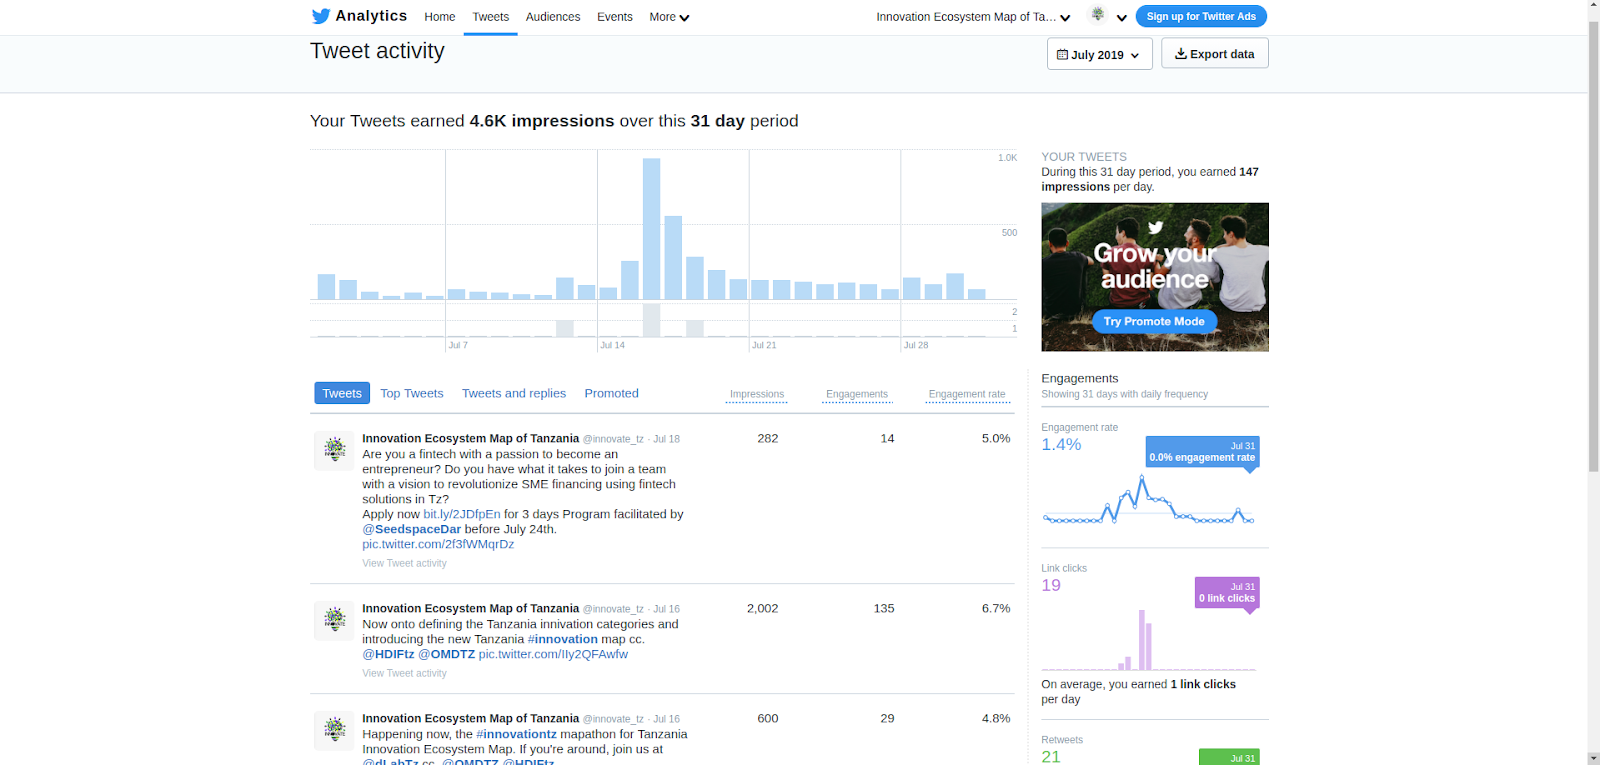
\includegraphics [width=1\textwidth]{tweet_activity.png}
\end{figure}

\newpage
\section{Conclusion}
From the feedback we have received during this quarter, we have generally learnt to invest more in engagement with the innovation community. This is through facilitating interconnection of the stakeholders within the ecosystem which can be achieved through events such as mapathons and workshops or various media channels.

\section{Financial Reporting}
Expenses breakdown:
\begin{figure}[h]
    \centering
    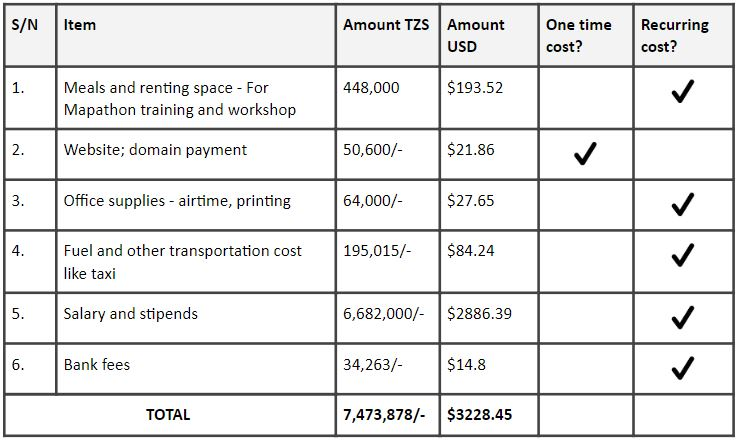
\includegraphics[width=0.9\textwidth]{images/finance.JPG}
\end{figure}


Second quarter opening and closing balance:
\begin{center}
	\begin{tabular}{|c|c|c|}
		\hline
		Item & TZS & USD \\
		\hline
		\rowcolor{Gray}
		Opening balance & 3,621,456/- & \$1,564.34 \\
	
		Amount advanced & 7,395,575/- & \$3,194.63 \\
		
		\rowcolor{Gray}
		Amount spent & 7,473,878/- & \$3,227.06 \\
		
		Balance in bank account + cash on hand & 3,543,153/- & \$1,530.51 \\
		\hline
	\end{tabular}
\end{center}

\end{document}
